\documentclass{beamer}
\usepackage{verbatim}
%\usepackage{enumitem}
\usetheme{Warsaw}
\setbeamertemplate{navigation symbols}{}
\renewcommand{\emph}{\textbf}
\title{Ch. 1 -- Descriptive Statistics and Overview}
\begin{document}
\begin{frame}
\begin{beamercolorbox}[rounded=true,wd=\textwidth,center]{title}
\usebeamerfont{title}\inserttitle
\end{beamercolorbox}%\begin{center}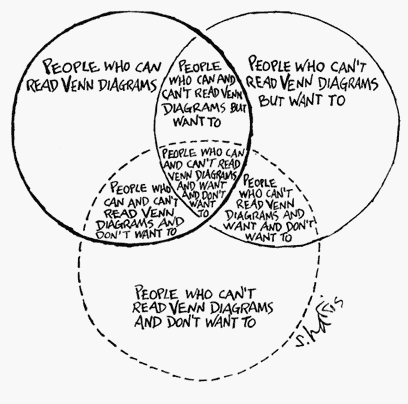
\includegraphics[scale=.4]{venn.png}
\vspace{1cm}
\begin{center}
\hspace*{-.7cm}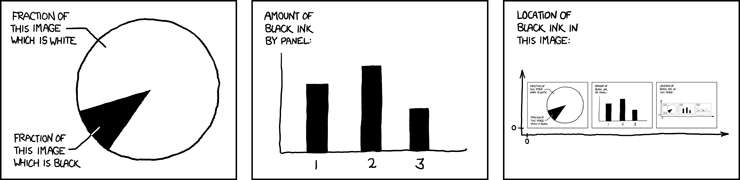
\includegraphics[scale=.52]{self_description.png}
\end{center}
\hfill\tiny xkcd.com
\end{frame} 

\begin{frame}{Example 1 -- Concrete Strength Data}
The following measurements of flexural strength (in MPa) were taken from 27 specimens of high-performance concrete obtained by using superplasticizers and certain binders\footnote{From ``Effects of Aggregates and Microfillers on the Flexural Properties of Concrete", \emph{Magazine of Concrete Research}, 1997: 81--98}:

\vspace{.5cm}
5.9,
6.3,
6.3,
6.5,
6.8,
6.8,
7.0,
7.0,
7.2,
7.3,
7.4,
7.6,
7.7,
7.7,
7.8,
7.8,
7.9,
8.1,
8.2,
8.7,
9.0,
9.7,
9.7,
10.7,
11.3,
11.6,
11.8

\begin{itemize}
\item How can we \emph{visualize} this distribution?
\item How can we quantify the \emph{center} of the distribution?
\item How can we quantify the \emph{spread} of the distribution?
\end{itemize}
\end{frame}

\begin{frame}{Dotplot}
One simple method of visualization is a \emph{dotplot} (or strip chart). The 27 observations are simply plotted on a line:
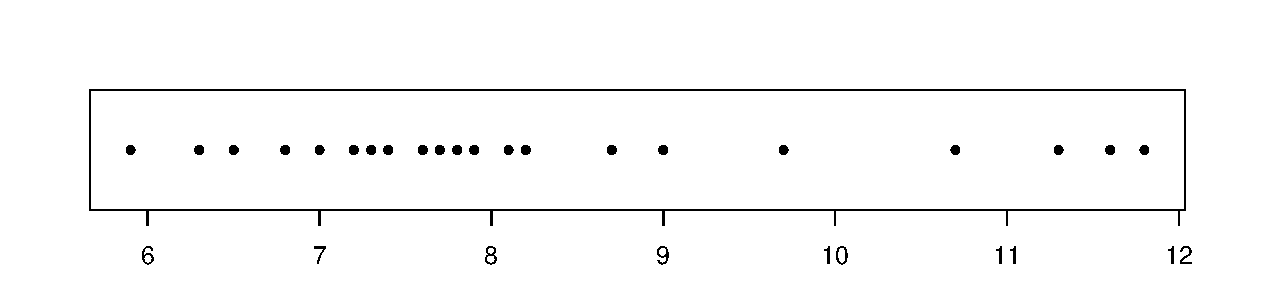
\includegraphics[scale=.5]{ch01_strength_dot.pdf}

\pause
Identical values may be represented by stacking the dots:
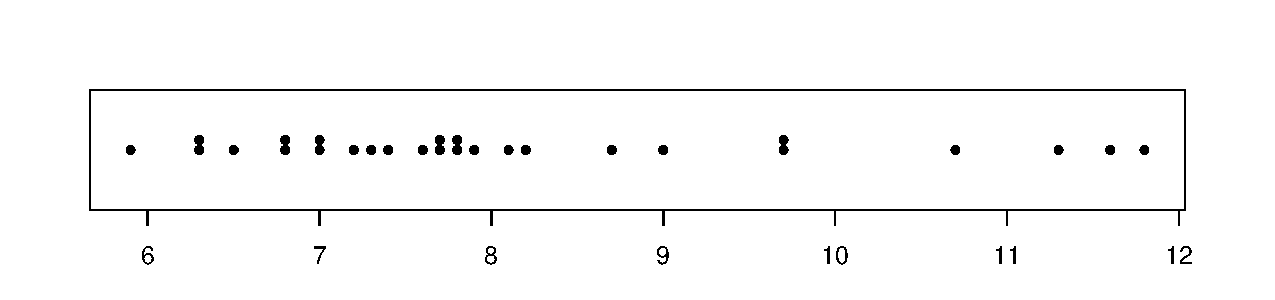
\includegraphics[scale=.5]{ch01_strength_dot_stack.pdf}
\end{frame}

\begin{frame}{Measures of center: Sample Mean and Median}
%Given data $x_1,\dots,x_n$, there are two common methods of quantifying the \emph{center} of the data:
\begin{enumerate}
\item The \emph{sample mean}: $$\overline{x} = \frac1n\sum_{i=1}^n x_i = \frac{x_1+\cdots+x_n}n$$
\pause
\item The \emph{sample median}: Sort the data from smallest to largest. If $n$ is odd, then the sample median $\tilde{x}$ is the middle observation in the list; if $n$ is even, then $\tilde{x}$ is the average of the two middle observations. Explicitly, if $x_1 \leq x_2 \leq \cdots \leq x_n$, 
$$\tilde{x} = \begin{cases}
x_{(n+1)/2} & \text{if $n$ is odd} \\
\frac12(x_{n/2} +x_{n/2+1}) & \text{if $n$ is even}
\end{cases}$$
\end{enumerate}
\pause
For example, given data 2, 3, 9, 11, 15, 17 we would have
\begin{align*}
\text{Sample mean: } &\overline{x}=\frac16(2+3+9+11+15+17)=9.5\\
\text{Sample median: }& \tilde{x}=\frac12(9+11)=10
\end{align*}
\end{frame}

\begin{frame}{Mean vs. Median}
The sample mean and sample median for the strength data are $\overline{x}=8.14$, $\tilde{x}=7.7$.
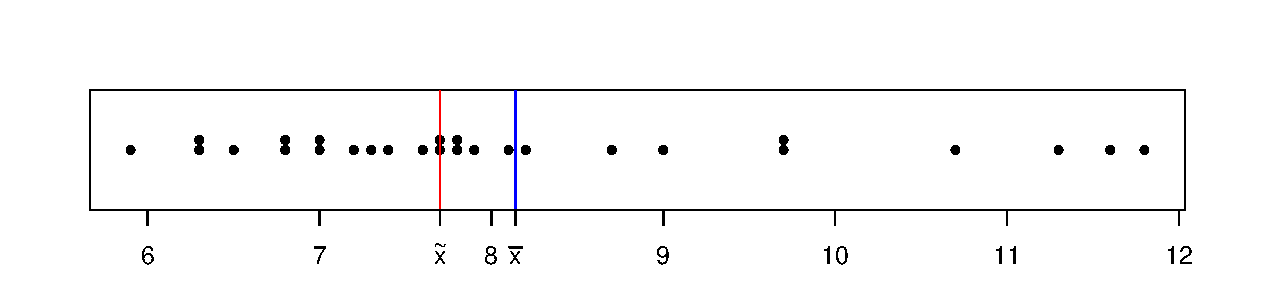
\includegraphics[scale=.5]{ch01_strength_dot_mm.pdf}
\begin{itemize}
\item The mean may be strongly influenced by a few extreme observations, whereas the median is \emph{robust} against such influence. 
\item If the largest measurement 11.8 were replaced 118, then the mean would increase to $\overline{x}=12.07$, while the median would remain $\tilde{x}=7.7$. 
\end{itemize}
\end{frame}

\begin{frame}{Sample Mean vs. Sample Median}
If the sample median is robust but the sample mean isn't, why use the mean?
\begin{itemize}
\pause\item In many cases, the sample mean is more \emph{efficient} than the sample median: it achieves greater accuracy with a smaller sample size.
\pause\item To address the sample mean's sensitivity to outliers, we may carefully check in advance to screen out any bad data.
\pause\item To achieve a balanced tradeoff between efficiency and robustness, there are hybrid approaches such as a \emph{trimmed mean}, e.g., discarding the top 10\% and bottom 10\% and then taking the sample mean of the remaining data.
\pause\item We'll discuss these issues in Chapter 6 (Point Estimation).
\end{itemize}

\end{frame}

\begin{frame}{Measure of Spread: Sample variance}
In addition to describing the center of the data (using the mean or median), we also want to describe how ``spread out" the data is. This can be measured using the \emph{sample variance}:
$$s^2 = \frac1{n-1}\sum_{i=1}^n(x_i-\overline{x})^2 = \frac{(x_1-\overline{x})^2+\cdots+(x_n-\overline{x})^2}{n-1}$$
\pause
The \emph{sample standard deviation} is the square root of the sample variance:
$$s = \sqrt{\frac1{n-1}\sum_{i=1}^n(x_i-\overline{x})^2} = \sqrt{\frac{(x_1-\overline{x})^2+\cdots+(x_n-\overline{x})^2}{n-1}}$$
\pause
Like the mean, the sample variance and sample standard deviation may be strongly influenced by extreme observations.
\end{frame}

\begin{frame}{Calculating the Sample Variance and Standard Deviation}
Given data 2, 3, 9, 11, 15, 17, we can calculate the sample variance (recall $\overline x=9.5$):
\pause\begin{align*}
s^2 &= \frac1{n-1}\sum_{i=1}^n(x_i-\overline{x})^2 = \frac{(x_1-\overline{x})^2+\cdots+(x_n-\overline{x})^2}{n-1} \\
\uncover<3->{ &= \tfrac{(2-9.5)^2+(3-9.5)^2+(9-9.5)^2+(11-9.5)^2+(15-9.5)^2+(17-9.5)^2}{6-1}} \\
\uncover<4->{ &= 37.5}
\end{align*}
\uncover<5->{
Now we can calculate the sample standard deviation:}
\uncover<6->{
$$ s = \sqrt{37.5} \approx 6.12$$}
\end{frame}

\begin{frame}{Robust Measure of Spread: Interquartile Range}
A robust measure of spread, called the \emph{interquartile range (IQR)}, is calculated as follows:
\begin{itemize}
\item Separate the data into the smaller half and larger half.\\
(Include the median $\tilde{x}$ in both halves if $n$ is odd.)
\pause\item The median of the smaller half is called the \emph{first quartile}, or lower fourth.
\pause\item The median of the larger half is called the \emph{third quartile}, or upper fourth. 
\pause\item Their difference is the \emph{interquartile range (IQR)}, or fourth spread:
$$\text{IQR} = \text{third quartile}-\text{first quartile}$$
\end{itemize}
\pause
Example: Given data 2,3,5,6,8,9,12,13,15 the median is $\tilde{x}=8$, the first quartile is 5, the third quartile is 12, and the interquartile range is 7.

\pause
\vspace{-.2in}\begin{center}
\begin{tabular}{r|cc}
& Efficient & Robust \\ \hline
Measure of center & $\overline{x}$ & $\tilde{x}$ \\
Measure of spread & $s$ & IQR
\end{tabular}
\end{center}

\end{frame}

\begin{frame}{Five-number summary and Boxplot}
\begin{tabular}{p{2.5in}p{2in}}
\begin{tabular}{p{2.5in}}
The \emph{five-number summary} consists of
\vspace{-.2in}\begin{enumerate}
\item The minimum observation
\item The first quartile %lower fourth
\item The median
\item The third quartile %upper fourth
\item The maximum observation
\end{enumerate}
For the concrete strength data: 
$$5.90, 7.00, 7.70, 8.85, 11.80$$

This is shown graphically in a \emph{boxplot}: The bottom and top of the box show the first and third quartiles; the horizontal line inside the box shows the median; the whiskers (dotted lines) extend to the minimum and maximum observations.
\end{tabular} &
\begin{tabular}{p{2in}}
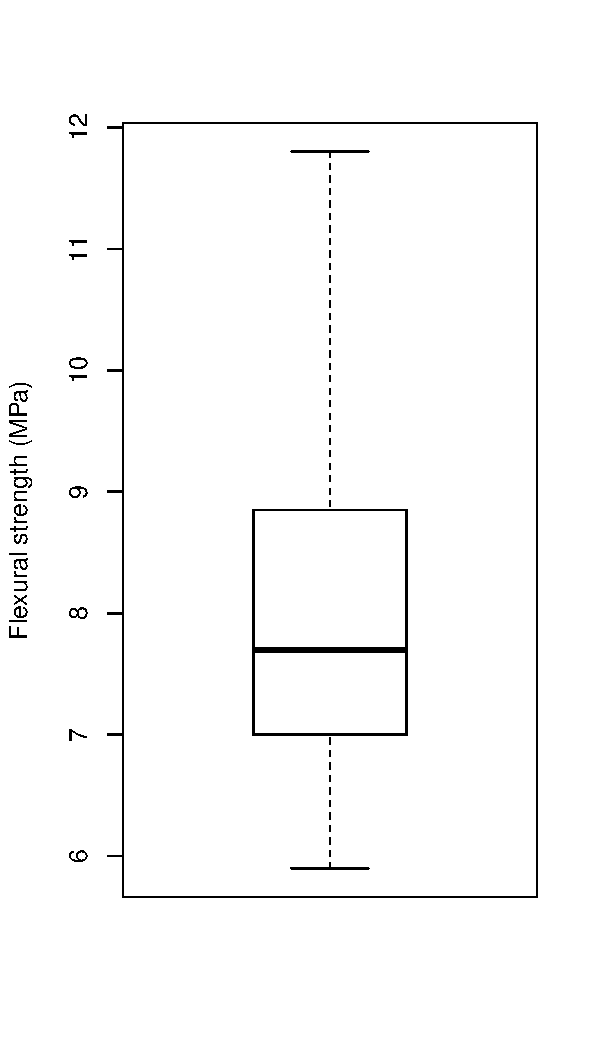
\includegraphics[scale=.4]{ch01_strength_boxplot.pdf}
\end{tabular}
\end{tabular}
\end{frame}

\begin{frame}{Example 2 -- Power Usage}
Power companies need information about customer usage to obtain accurate forecasts of demands. Investigators from a power company determined energy consumption (in BTU) for a sample of 90 homes over a fixed time interval:

\vspace{.5cm}
2.97,
4.00,
5.20,
5.56,
5.94,
5.98,
6.35,
6.62,
6.72,
6.78,
6.80,
6.85,
6.94,
7.15,
7.16,
7.23,
7.39,
7.62,
7.62,
7.69,
7.73,
7.87,
7.93,
8.00,
8.26,
8.29,
8.37,
8.47,
8.56,
8.58,
8.61,
8.67,
8.69,
8.81,
9.07,
9.27,
9.37,
9.43,
9.52,
9.58,
9.60,
9.76,
9.82,
9.83,
9.83,
9.84,
9.96,
10.04,
10.21,
10.28,
10.28,
10.30,
10.35,
10.36,
10.40,
10.49,
10.50,
10.64,
10.95,
11.09,
11.12,
11.21,
11.29,
11.43,
11.62,
11.70,
11.70,
12.16,
12.19,
12.28,
12.31,
12.62,
12.69,
12.71,
12.91,
12.92,
13.11,
13.38,
13.42,
13.43,
13.47,
13.60,
13.96,
14.24,
14.35,
15.12,
15.24,
16.06,
16.90,
18.26
\end{frame}


\begin{frame}{Example 2 -- Power Usage}
%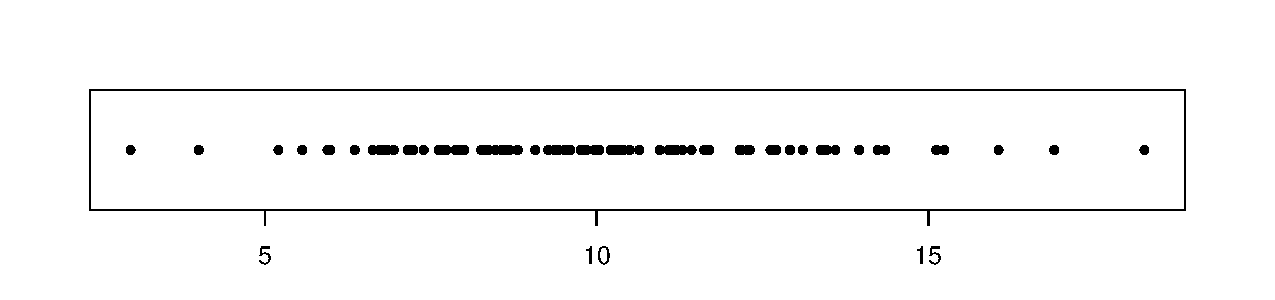
\includegraphics[scale=.5]{ch01_power_dot.pdf}
The dotplot is less effective here: many dots are packed close together, making it difficult to see where the dots are most concentrated:

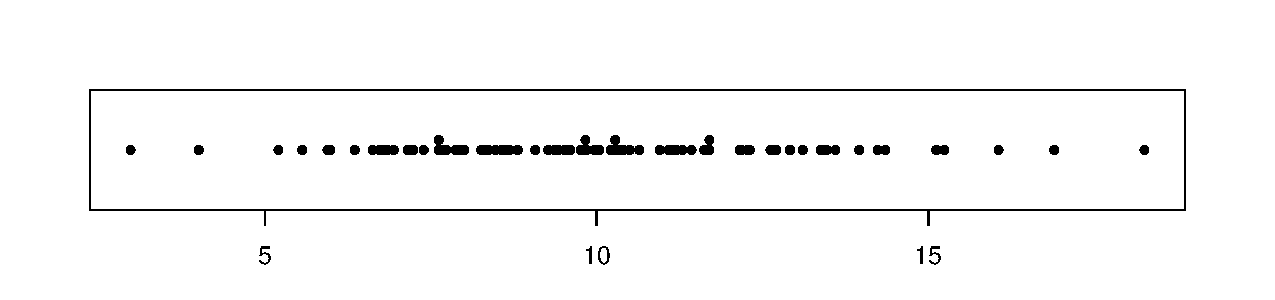
\includegraphics[scale=.5]{ch01_power_dot_stack.pdf}
\end{frame}

\begin{frame}{Histogram}
A \emph{histogram} is constructed by grouping the data into bins of equal width and counting the number of observations within each bin:

\begin{tabular}{p{2.7in}p{1.4in}}
\begin{tabular}{l}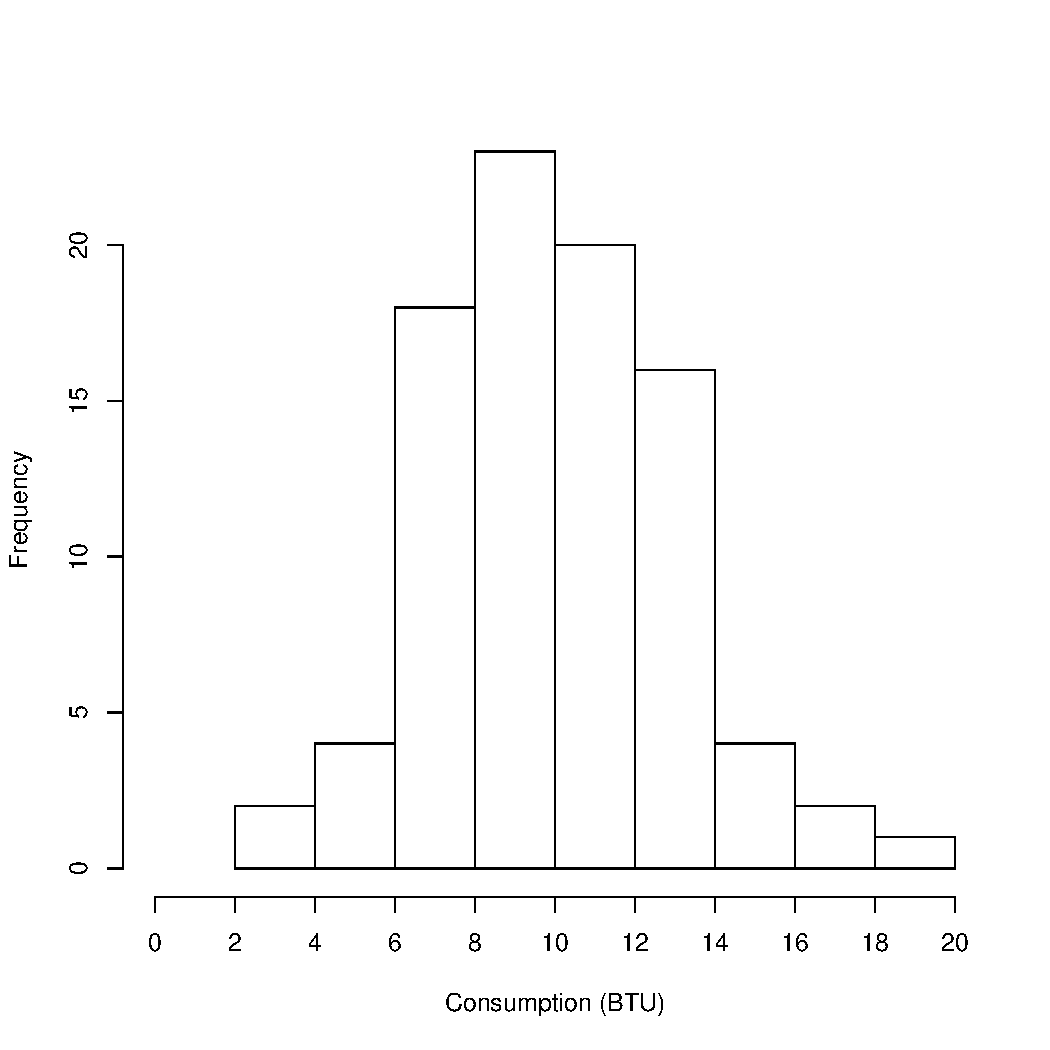
\includegraphics[scale=.4]{ch01_power_hist.pdf}\end{tabular}&\begin{tabular}{p{1.4in}}
Here the bins are the intervals (0,2], (2,4], (4,6], (6,8], \dots, (16,18], (18,20].

%\vspace{.1in}
%This histogram appears \emph{symmetric}, i.e., the left half looks like a mirror image of the right half. 
%
%\vspace{.1in}
%It is \emph{unimodal} in that there is a single peak.
\end{tabular}
\end{tabular}
\end{frame}

\begin{frame}{Normal Distribution}
This histogram appears to be a fairly close fit to the symmetric, bell-shaped density curve of a \emph{normal distribution}:
\begin{center}
\vspace{-.5cm}
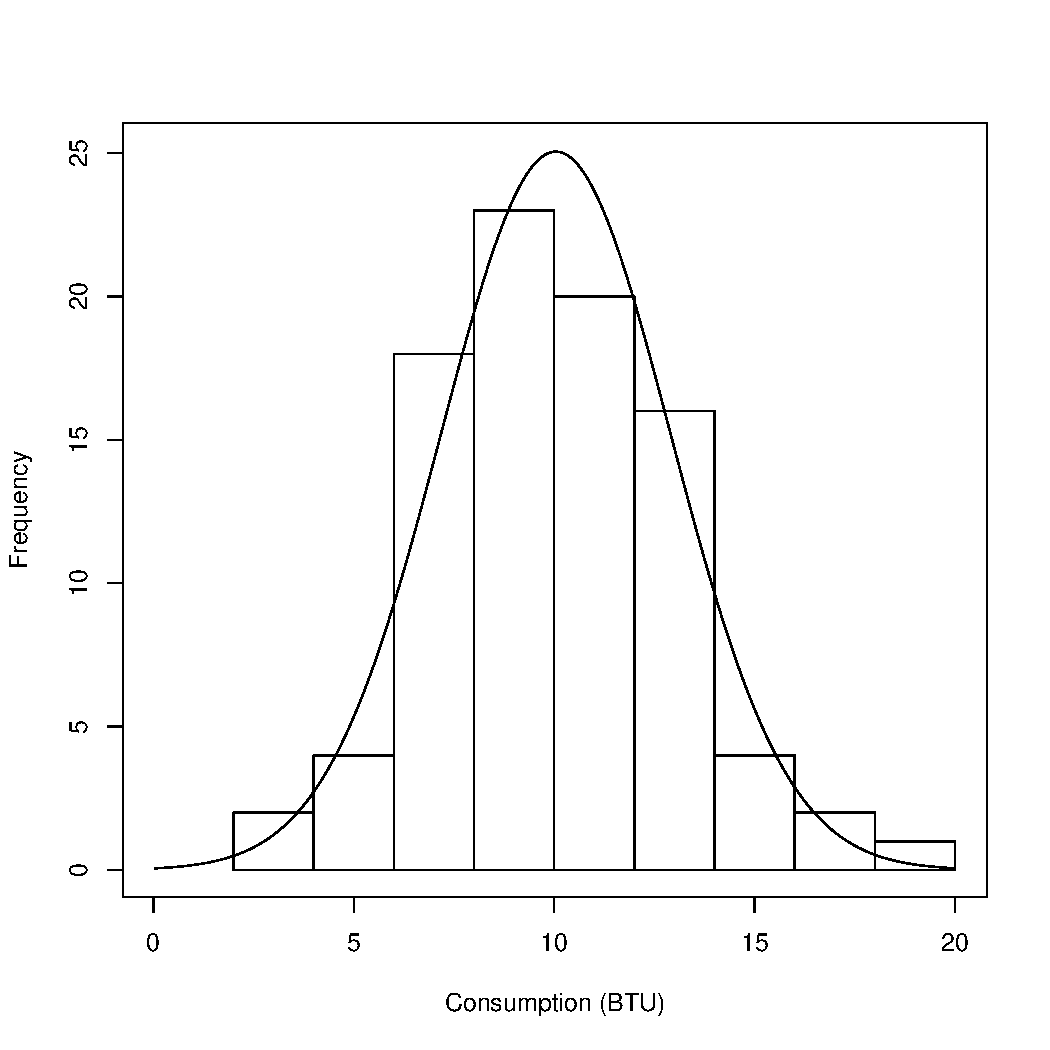
\includegraphics[scale=.35]{ch01_power_normal.pdf}
\end{center}
Normal distributions are very common in statistics and will be discussed in Chapter 4.
\end{frame}

%\begin{frame}{Weibull Distribution}
%In contrast, the concrete strength data appears asymmetric and does not seem to fit a normal distribution. A better fit is provided by a \emph{Weibull distribution}.
%\begin{center}
%\vspace{-.5cm}
%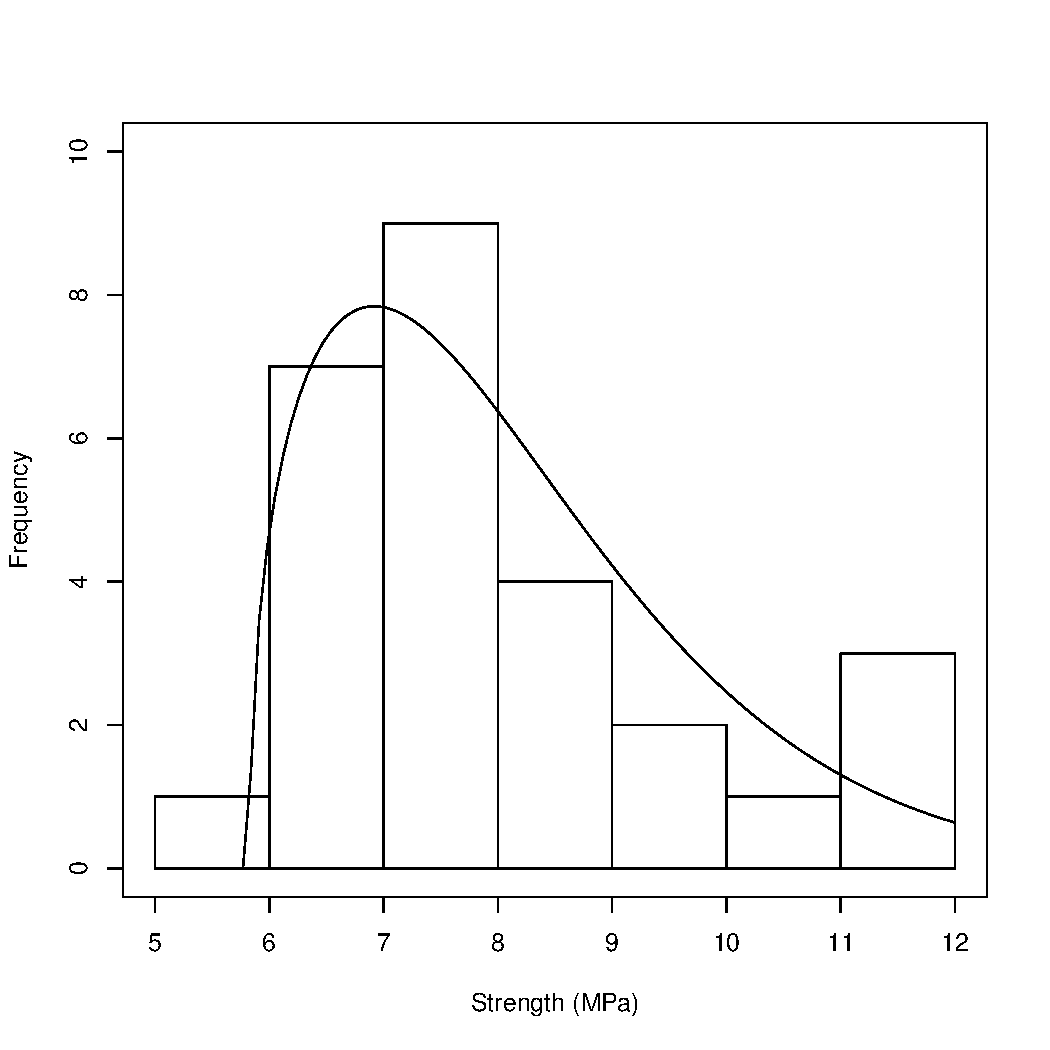
\includegraphics[scale=.35]{ch01_strength_weib.pdf}
%\end{center}
%\end{frame}

%\begin{frame}{Histogram}
%We may also display a histogram of the concrete strength data:
%
%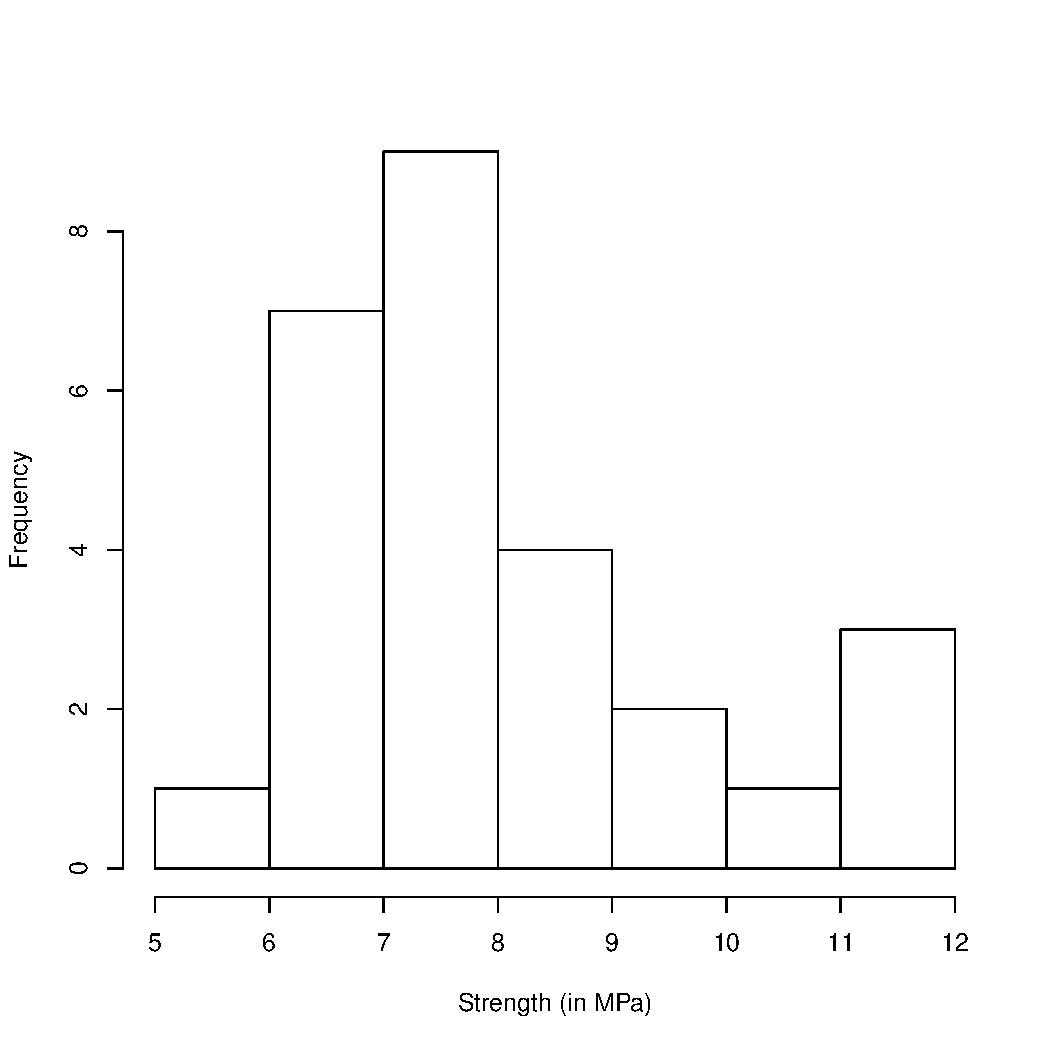
\includegraphics[scale=.35]{ch01_strength_hist.pdf}
%
%Here the histogram appears \emph{bimodal}, having two peaks.
%\end{frame}

\begin{frame}[fragile]{Stem-and-leaf diagram}
\vspace{-.1in}
\begin{tabular}{p{1.7in}p{2.5in}}
\begin{tabular}{p{1.7in}}
\begin{verbatim}
   3 | 0
   4 | 0
   5 | 269
   6 | 03678889
   7 | 2224667799
   8 | 03345666778
   9 | 134456688888
  10 | 0023333445569
  11 | 11234677
  12 | 223367799
  13 | 144456
  14 | 023
  15 | 12
  16 | 19
  17 | 
  18 | 3
\end{verbatim}
\end{tabular}
& 
\begin{tabular}{p{2.5in}}
A \emph{stem-and-leaf diagram} is constructed by grouping the data according to their first one or two digits (the \emph{stem}), shown on the left part of the diagram, while the remaining digit (the \emph{leaf}) is displayed on the right.

\vspace{.1in}
Here the first few measurements are 3.0, 4.0, 5.2, 5.6, 5.9, 6.0, 6.3, etc.

\vspace{.1in}
A stem-and-leaf diagram is similar to a ``sideways" histogram. It is visually less appealing but provides more precise information about the data.
\end{tabular}
\end{tabular}
\end{frame}


\begin{frame}{Population vs. Sample}
\begin{itemize}
\item A \emph{population} is a group that we want to study.
\pause\item A \emph{sample} is a subset of a population that is observed and measured.
\pause\item For example, Gallup regularly polls American adults about their opinions on various topics. The relevant \textit{population} consists of the group of all American adults, consisting of approximately 240 million people. For any given poll, however, the \textit{sample} typically consists of at most a few thousand people who are actually contacted by Gallup and polled.
\pause\item In the concrete-strength example, only 27 specimens of concrete were tested. The 27 specimens form the \textit{sample} which the researchers directly measure. The \textit{population} consists of all such concrete specimens have been or could be formed by the same process and under the same conditions.
\end{itemize}
\end{frame}
\begin{frame}{Estimation: Parameters vs. Statistics}
\begin{itemize}
\item A \emph{parameter} is a quantity which describes a population. %, e.g., the population mean $\mu$.
\pause\item A \emph{statistic} is a quantity computed from sample data, used to estimate a population parameter. %e.g., the sample mean $\overline{x}$. 
\pause\item Gallup ran a poll in December 2014, asking 805 American adults, ``Do you approve or disapprove of the way Congress is handling its job?"
16\% said ``Yes". This 16\% is a \textit{statistic}, called the \emph{sample proportion~$\hat{p}$}.
The percentage of all American adults who would answer ``Yes" is a parameter, called the \emph{population proportion~$p$}. The parameter $p$ is not known but is probably within a few percentage points of 16\%.
\pause\item In the concrete-strength example, the 27 specimens had an average strength of 8.14 MPa. This is a \textit{statistic}, the \emph{sample~mean~$\overline{x}$}. The mean strength of all potential specimens is a \textit{parameter}, the \emph{population~mean~$\mu$}. Likewise, the sample standard deviation $s$ is a statistic, estimating the \emph{population standard deviation $\sigma$}.
%\item We will discuss the theory of estimation in Ch. 6.
\end{itemize}
\end{frame}
\begin{frame}{Statistical Inference}
\emph{Statistical inference} is the method of drawing \textit{probabilistic} conclusions about a population based on sample data. 
\begin{itemize}
\pause\item A \emph{confidence interval} is a range of values containing a population parameter, with a specific degree of confidence. For example, in the case of the Gallup poll, we can say with 95\% confidence that between 12\% and 20\% of American adults approved of the way Congress was handling its job.
We will discuss confidence intervals in Ch.\@ 7 and Ch.\@ 9.
\pause\item A \emph{hypothesis test} is a way to test whether a theory is consistent with the data or not. 
For example, in the Gallup poll, one might hypothesize that a different proportion of Republicans would answer ``Yes" compared to Democrats. However, the data gives no significant support for this ($P=0.53$).  We will discuss hypothesis tests in Ch.~8.
\pause \item We cannot be certain that the conclusions of statistical inference are correct, but we can quantify the degree of uncertainty using \textit{probability} (Chs.\@ 2 through 5).
\end{itemize}
\end{frame}

%\begin{frame}{Statistical Inference: Confidence Intervals}
%\begin{itemize}
%\item In the concrete strength data, based on 27 specimens, the sample mean was $\overline{x}=8.14$. 
%\pause\item If the process were repeated under the same conditions, creating a new sample of 27 specimens, the new sample may have a somewhat different sample mean.
%\pause\item The sample mean $\overline{x}$ is only an estimate of the true \emph{population mean} $\mu$.
%\pause\item The accuracy of this estimate may be quantified using a \emph{confidence interval}: In this case, given the sample of 27 specimens, we can say with 95\% confidence that the population mean $\mu$ is between 7.51 and 8.77.
%\end{itemize}
%\begin{center}
%\vspace{-1cm}
%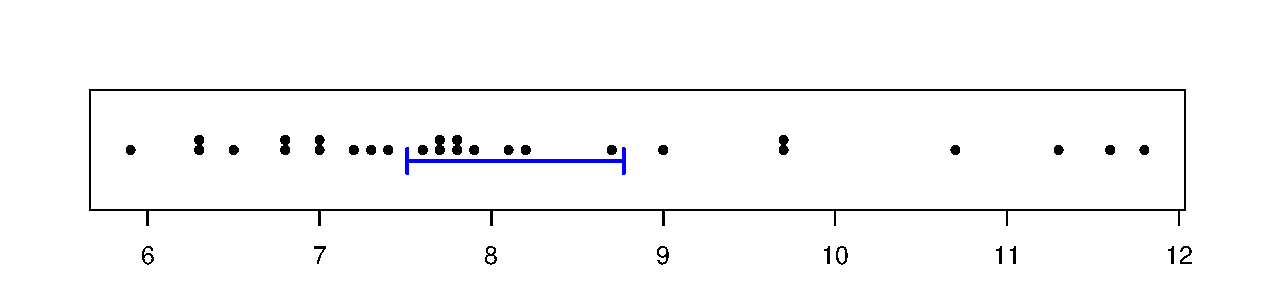
\includegraphics[scale=.55]{ch01_strength_conf.pdf}
%\end{center}
%\end{frame}
%
%\begin{frame}{Statistical Inference: Hypothesis Tests}
%\begin{itemize}
%\item Suppose a second method of producing high-strength concrete is tested: 30 specimens have a sample mean flexural strength of $\overline{y}=8.90$, compared to $\overline{x}=8.14$ for the original method.
%\pause\item Does the second method produce stronger concrete? Or could the difference be due to chance?
%\pause\item To answer this, we need to know the sample standard deviations of the two samples: $s_1=1.66$, $s_2=1.91$.
%\pause\item The appropriate hypothesis test (two-sample t test) gives a \emph{$P$-value} of .06, which means that if there is no difference in the population means of the two methods, there is only a 6\% chance that the sample means $\overline{x}$ and $\overline{y}$ would differ by as much as they did.
%\pause\item This provides some evidence (but not strong evidence) that the second method outperforms the first in mean flexural strength.
%\end{itemize}
%\end{frame}

% Shapiro-Wilk
%\begin{frame}{Statistical Inference: Hypothesis Tests}
%Based on the histogram, we remarked that the concrete strength data did not appear to have a normal distribution. However, appearances can be misleading, especially in small samples.
%\begin{center}
%\vspace{-.5cm}
%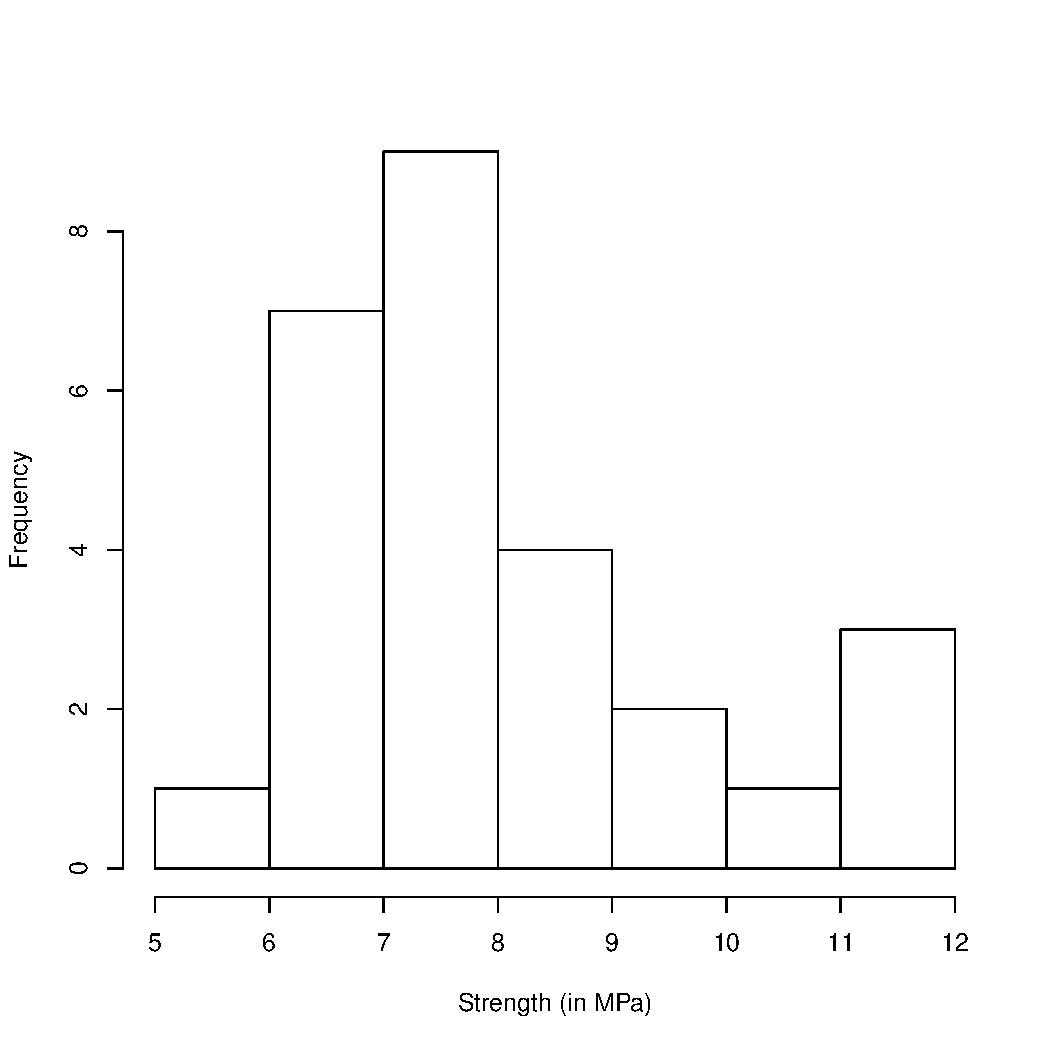
\includegraphics[scale=.3]{ch01_strength_hist.pdf}
%\end{center}
%A normality test (Shapiro-Wilk test) gives a P-value of .008, providing strong evidence that indeed the data is not normal.
%\end{frame}

% Birth gender example
%
%\begin{frame}{Categorical vs. Numerical Variables}
%Consider the population of current U of U students.
%
%\begin{itemize}
%\item \textbf{Categorical} variables: college major, gender, race
%\item \textbf{Numerical} variables: GPA, height, weight, income, age
%\end{itemize}
%
%\end{frame}

% Representation of categorical variables as 0-1 numerical.
% mean = proportion.

\begin{frame}{Key concepts}
\begin{itemize}

\item Ways to display the distribution of a numerical variable:
\begin{itemize}
\item dotplot, boxplot, histogram, stem-and-leaf diagram
\end{itemize}
\item Measures of center: sample mean, sample median
\item Measures of spread: sample variance, sample standard deviation, interquartile range
\item Statistical inference: using \textit{sample} data to draw probabilistic conclusions about a broader 
\textit{population}.
\begin{itemize}
\item Sample \textit{statistics} are used to estimate population \textit{parameters}.
\end{itemize}

\vspace{.1in}
\begin{center}\begin{tabular}{l|l}
Parameter & Statistic \\ \hline
population mean $\mu$ & sample mean $\overline{x}$ \\
population standard deviation $\sigma$ & sample standard deviation $s$ \\
population proportion $p$ & sample proportion $\hat{p}$
\end{tabular}
\end{center}
\end{itemize}
\end{frame}

\end{document}
